\subsection{Описание схемы БД}
Организация базы данных, используемой сервисом, представлена на рис.~\ref{db-scheme}.

Таблица ''application\_entity'' содержит записи с информацией об известных системе приложениях.
Описание полей сущности представлено в табл.~\ref{db-scheme-app}.

Таблица ''kubernetes\_config\_entity'' содержит записи с информацией о параметрах подключения к платформе ''Kubernetes'', а так же о конкретном приложении под управлением данной платформы.
Описание полей сущности представлено в табл.~\ref{db-scheme-kub}.

Таблица ''open\_nebula\_config\_entity''  содержит записи с информацией о параметрах подключения к платформе ''OpenNebula'', а так же о конкретном приложении под управлением данной платформы.
Описание полей сущности представлено в табл.~\ref{db-scheme-one}.

\begin{figure}[hbtp]
    \caption{Схема базы данных}
    \label{db-scheme}
    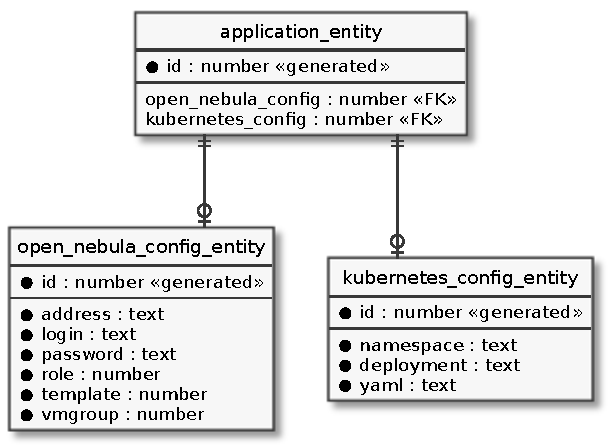
\includegraphics[width=13cm]{img/db-scheme.pdf}
\end{figure}

\begin{table}[hbtp]
    \caption{Описание полей сущности ''application\_entity''}
    \label{db-scheme-app}
    \begin{tabularx}{\linewidth}{l X}
        \textbf{Имя} & \textbf{Описание} \\
        \hline
        id & Первичный ключ сущности, уникальное число для идентификации записи. \\
        \hline
        kubernetes\_config & Первичный ключ сущности ''kubernetes\_config\_entity'' для связи приложения и его конфигурации в системе ''Kubernetes''. Может отсутствовать, если это приложение сконфигурировано в ''OpenNebula''. \\
        \hline
        open\_nebula\_config & Первичный ключ сущности ''open\_nebula\_config\_entity'' для связи приложения и его конфигурации в системе ''OpenNebula''. Может отсутствовать, если это приложение сконфигурировано в ''Kubernetes''. \\
    \end{tabularx}
\end{table}

\begin{table}[hbtp]
    \caption{Описание полей сущности ''kubernetes\_config\_entity''}
    \label{db-scheme-kub}
    \begin{tabularx}{\linewidth}{l X}
        \textbf{Имя} & \textbf{Описание} \\
        \hline
        id & Первичный ключ сущности, уникальное число для идентификации записи. \\
        \hline
        namespace & Имя того namespace ''Kubernetes'', в котором развёрнуто управляемое приложение. \\
        \hline
        deployment & Имя того deployment ''Kubernetes'', к которому относится управляемое приложение. \\
        \hline
        yaml & Конфигурация подключения к API ''Kubernetes'' в формате ''YAML'', эту конфигурацию ещё называют ''kube config''. \\
    \end{tabularx}
\end{table}

\begin{table}[hbtp]
    \caption{Описание полей сущности ''open\_nebula\_config\_entity''}
    \label{db-scheme-one}
    \begin{tabularx}{\linewidth}{l X}
        \textbf{Имя} & \textbf{Описание} \\
        \hline
        id & Первичный ключ сущности, уникальное число для идентификации записи. \\
        \hline
        address & URL, по которому расположен XML RPC API платформы ''OpenNebula''. \\
        \hline
        login & Логин пользователя. \\
        \hline
        password & Пароль пользователя. \\
        \hline
        role & Идентификатор роли внутри группы ВМ, к которой относится управляемое приложение. \\
        \hline
        template & Идентификатор шаблона VM, согласно которому будут создаваться новые ВМ управляемого приложения. \\
        \hline
        vmgroup & Идентификатор группы ВМ, к которой относится управляемое приложение. \\
    \end{tabularx}
\end{table}

\FloatBarrier